\section{Projection of the Measurement}
\subsection{Kinematic Coverage}
\begin{figure}[!ht]
 \begin{center}
      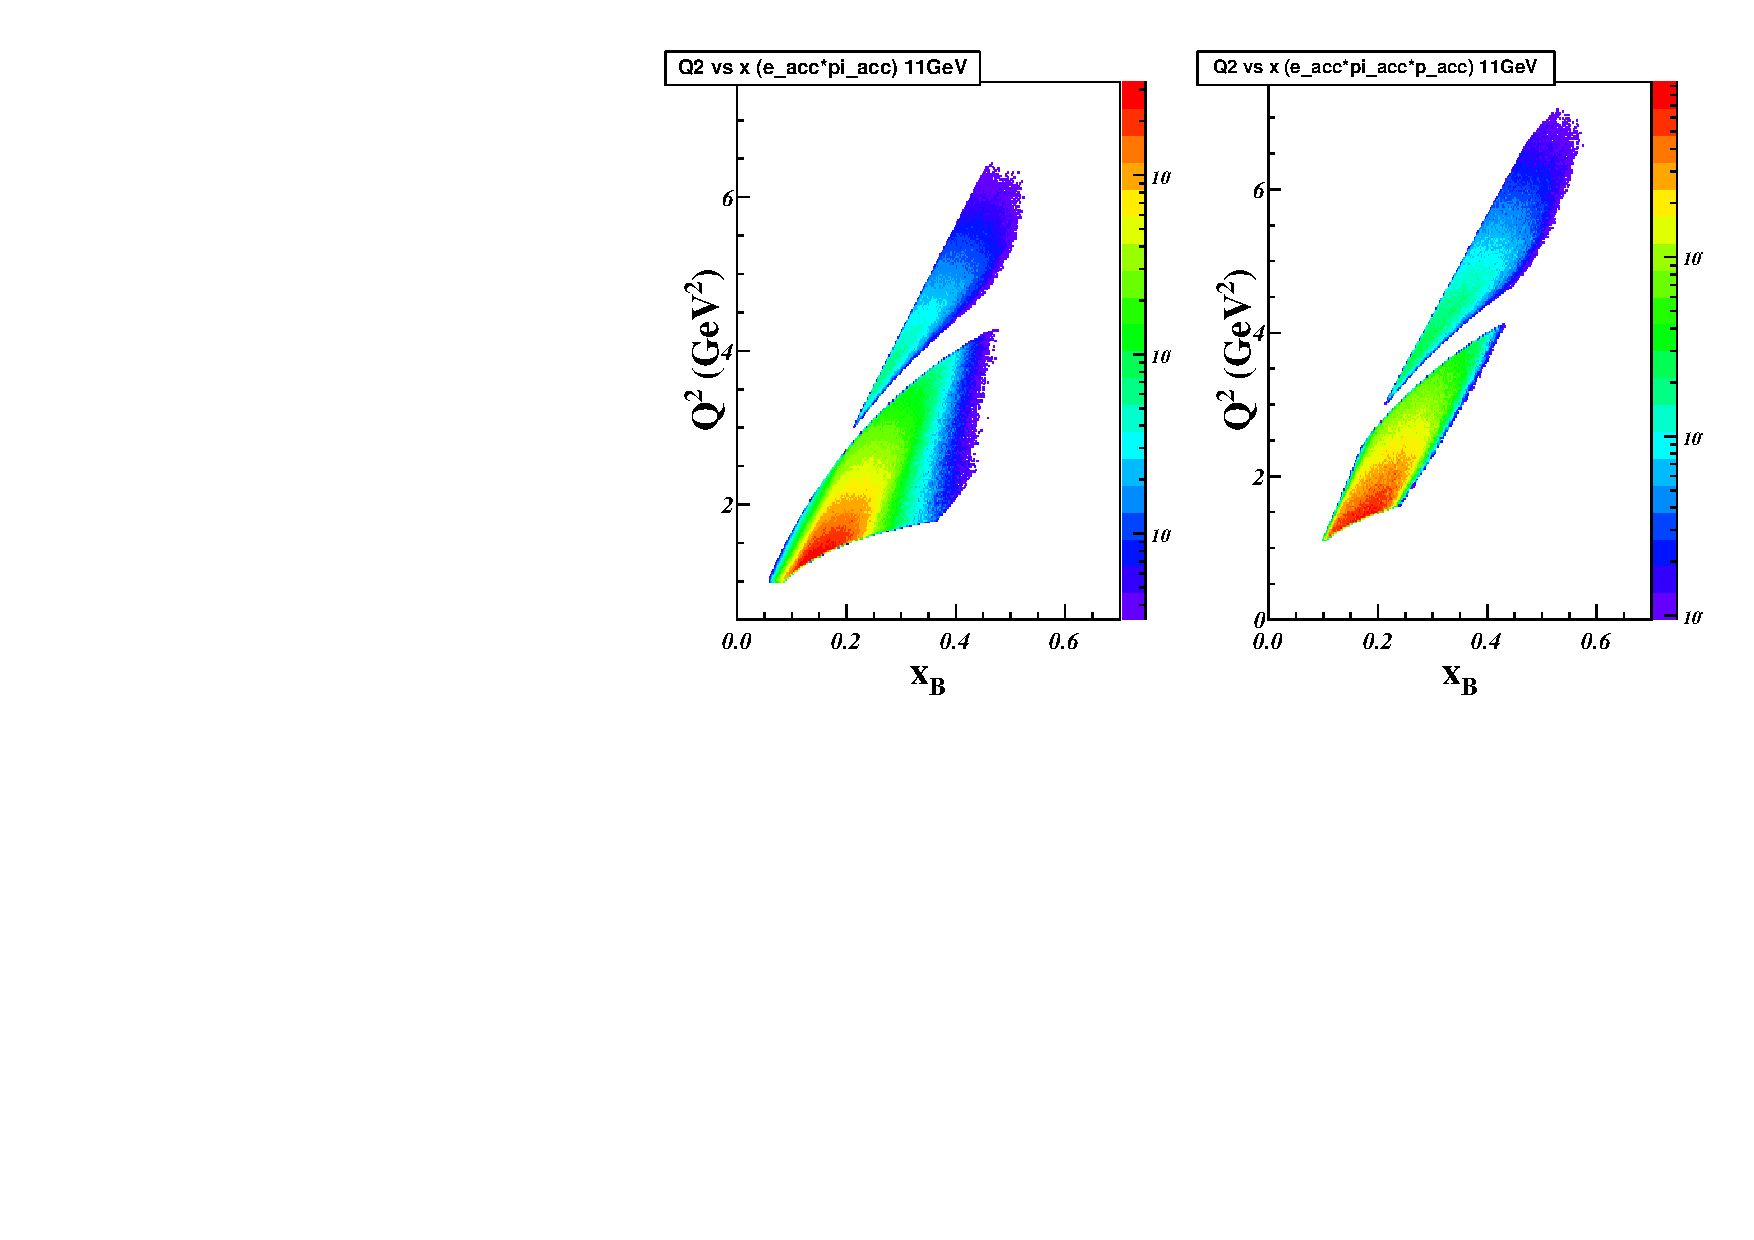
\includegraphics[type=pdf, ext=.pdf,read=.pdf,width=0.6\textwidth]{./figures/E11_Q2_x_epip_Q2gt1}
 \caption[The kinematic coverage at different acceptances]{\footnotesize{The kinematic coverage at different acceptances at $11~GeV$. The left plot shows the coverage when detecting all recoil protons, while the right plot shows the coverage with proton detection by existing SoLID detectors. Colors correspond to rates (Hz) in log scale.}}
  \label{kin_cor}
  \end{center}
\end{figure}

%\begin{figure}[!ht]
% \begin{center}
%    \subfloat[w/ $\mathrm{Q^{2}>1~GeV^{2}}$ cut]{
%      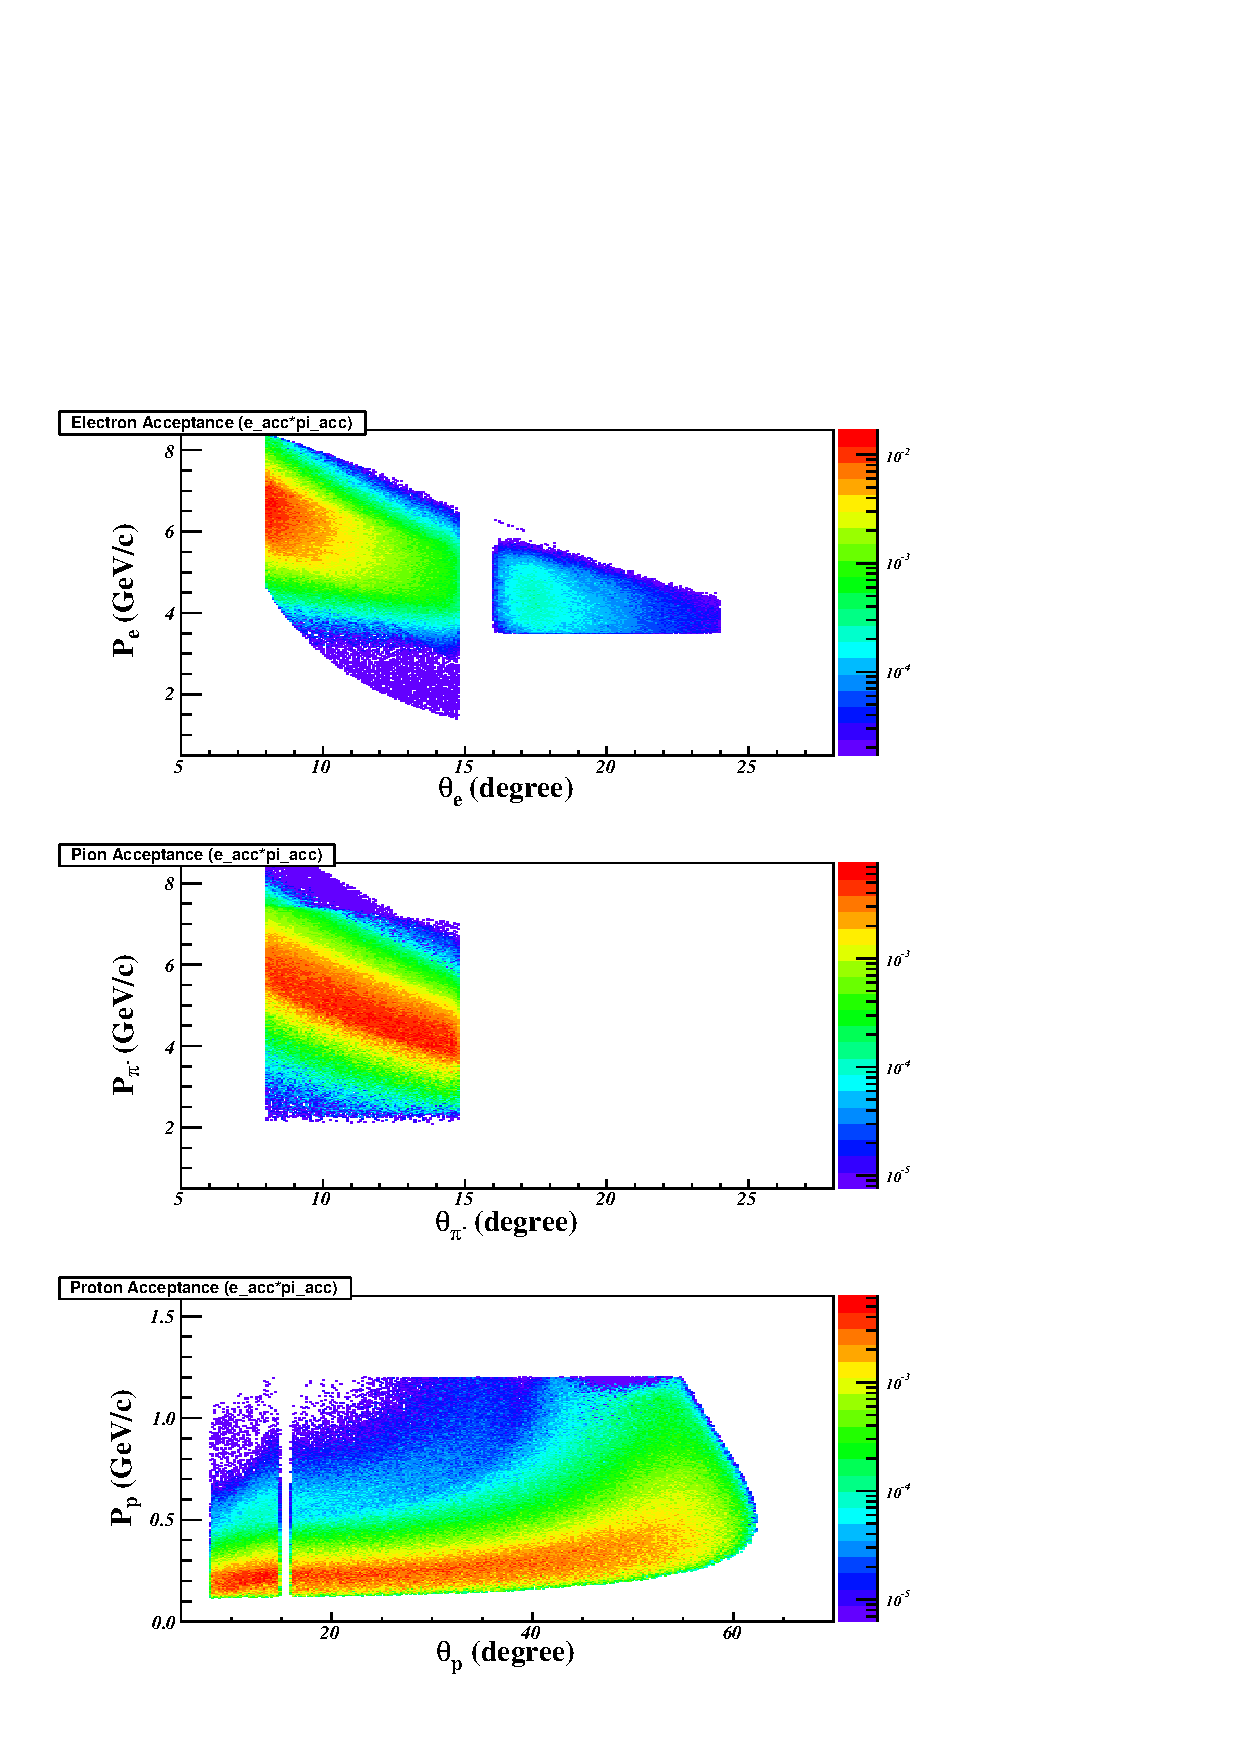
\includegraphics[type=pdf, ext=.pdf,read=.pdf,width=0.35\textwidth]{./figures/E11_acc_epi}
%    }
%     \subfloat[w/ $\mathrm{Q^{2}>4~GeV^{2}}$ cut]{
%      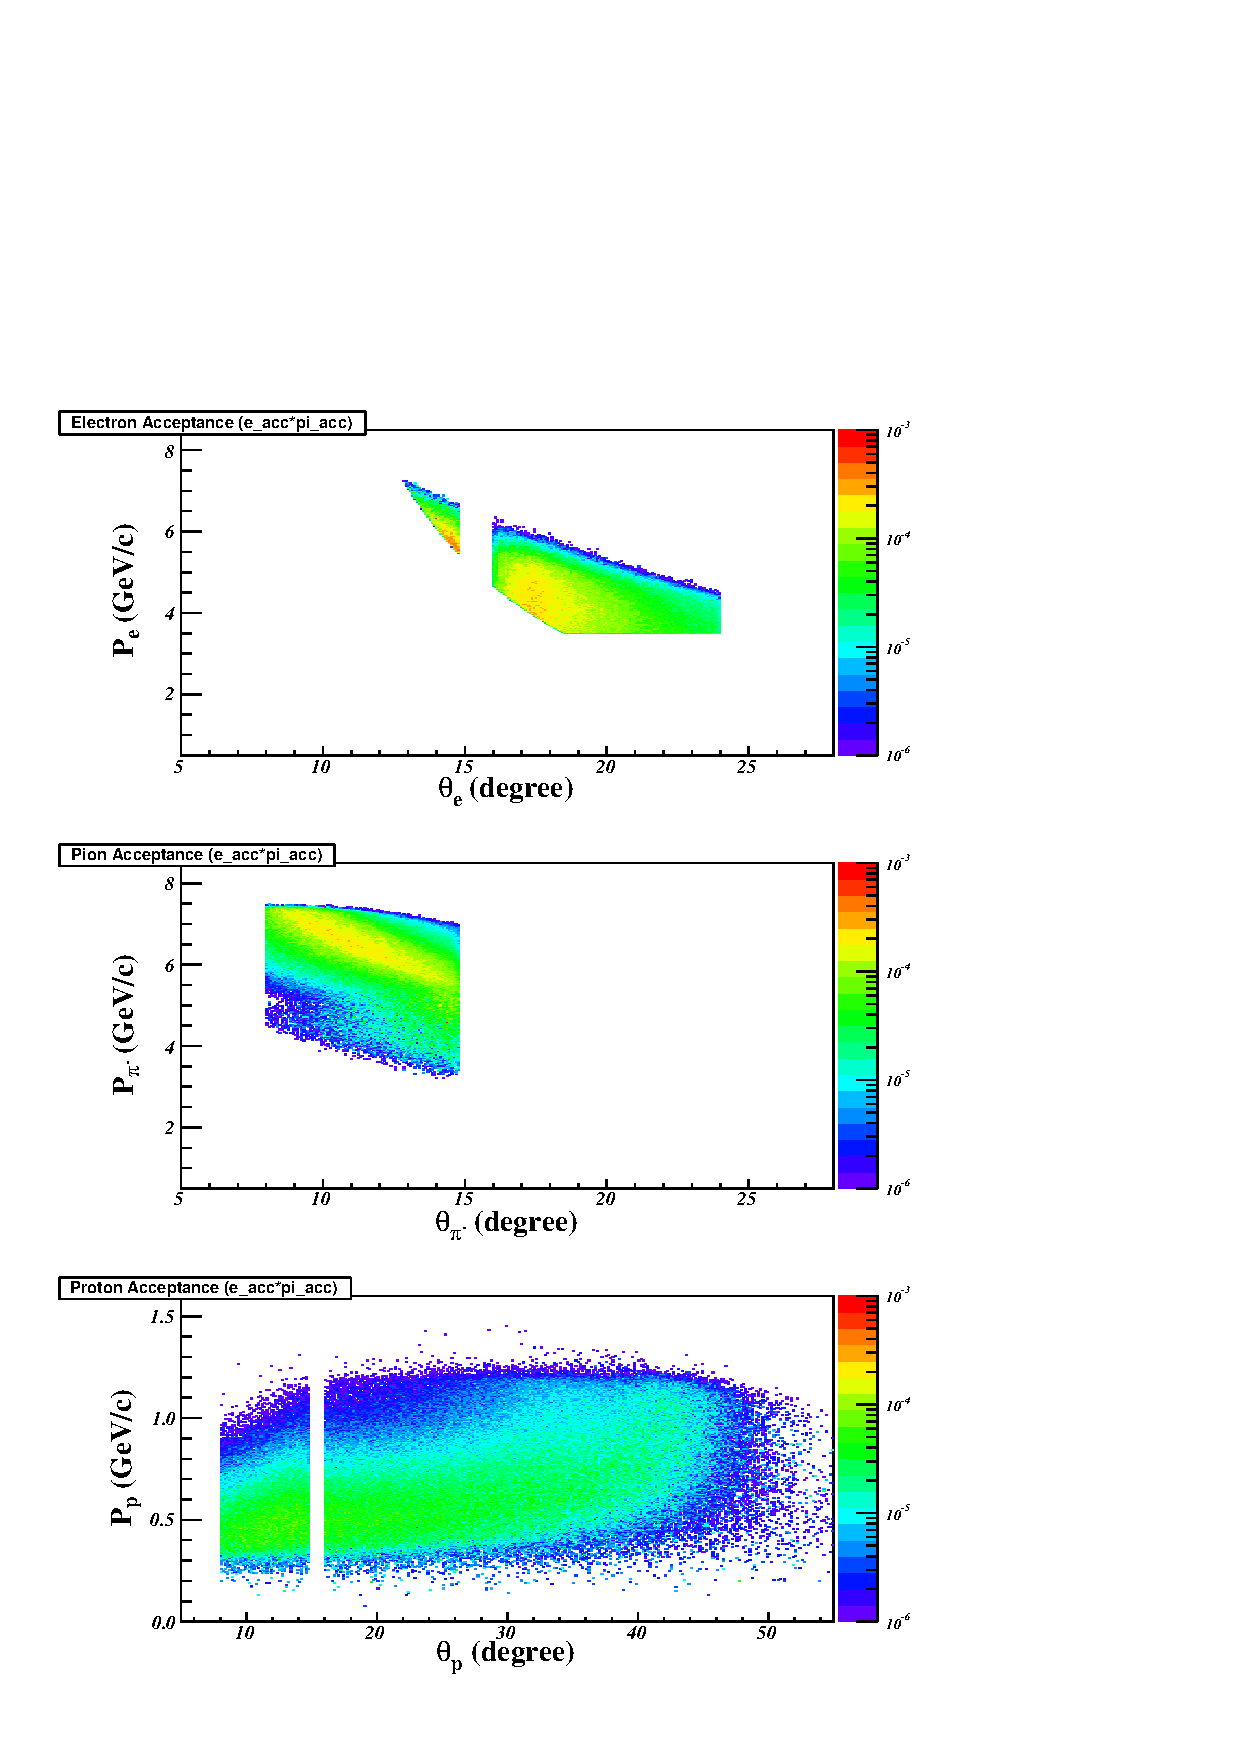
\includegraphics[type=pdf, ext=.pdf,read=.pdf,width=0.35\textwidth]{./figures/E11_acc_epi_Q2gt4}
%    }
%   \caption[The acceptance of the momenta and scattering angles for electrons, $\pi^{-}$ and protons]{\footnotesize{The acceptance of the momenta and polar angles at two different $\mathrm{Q^{2}}$ cuts. In each panel, the top, middle and bottom plots are for electrons, $\pi^{-}$ and protons, respectively. The distribution of protons is given by assuming we detect all recoil protons. Colors correspond to rates (Hz) in log scale.}}
%  \label{p_theta}
%  \end{center}
%\end{figure}
%\begin{figure}[!ht]
% \begin{center}
%    \subfloat[w/ $\mathrm{Q^{2}>1~GeV^{2}}$ cut]{
%      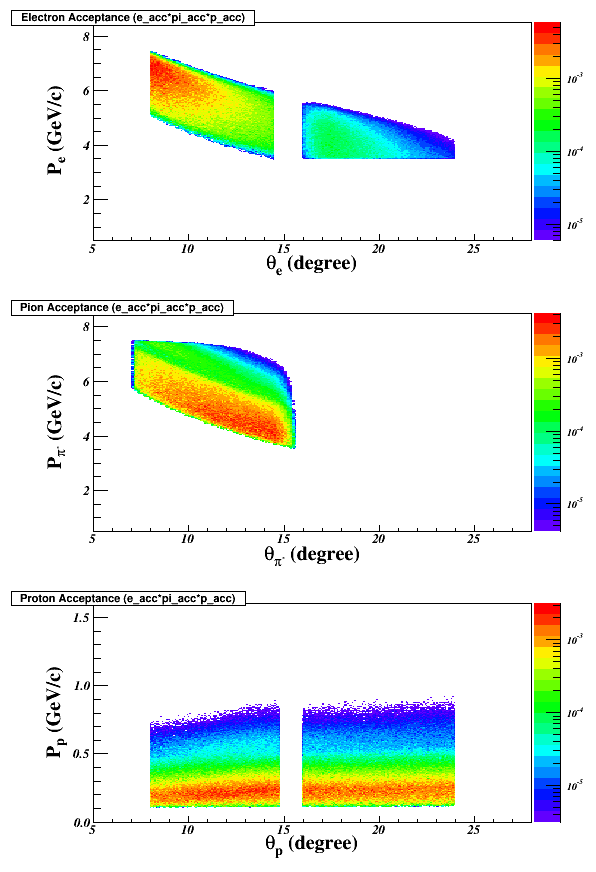
\includegraphics[type=pdf, ext=.pdf,read=.pdf,width=0.35\textwidth]{./figures/E11_acc_epip}
%    }
%     \subfloat[w/ $\mathrm{Q^{2}>4~GeV^{2}}$ cut]{
%      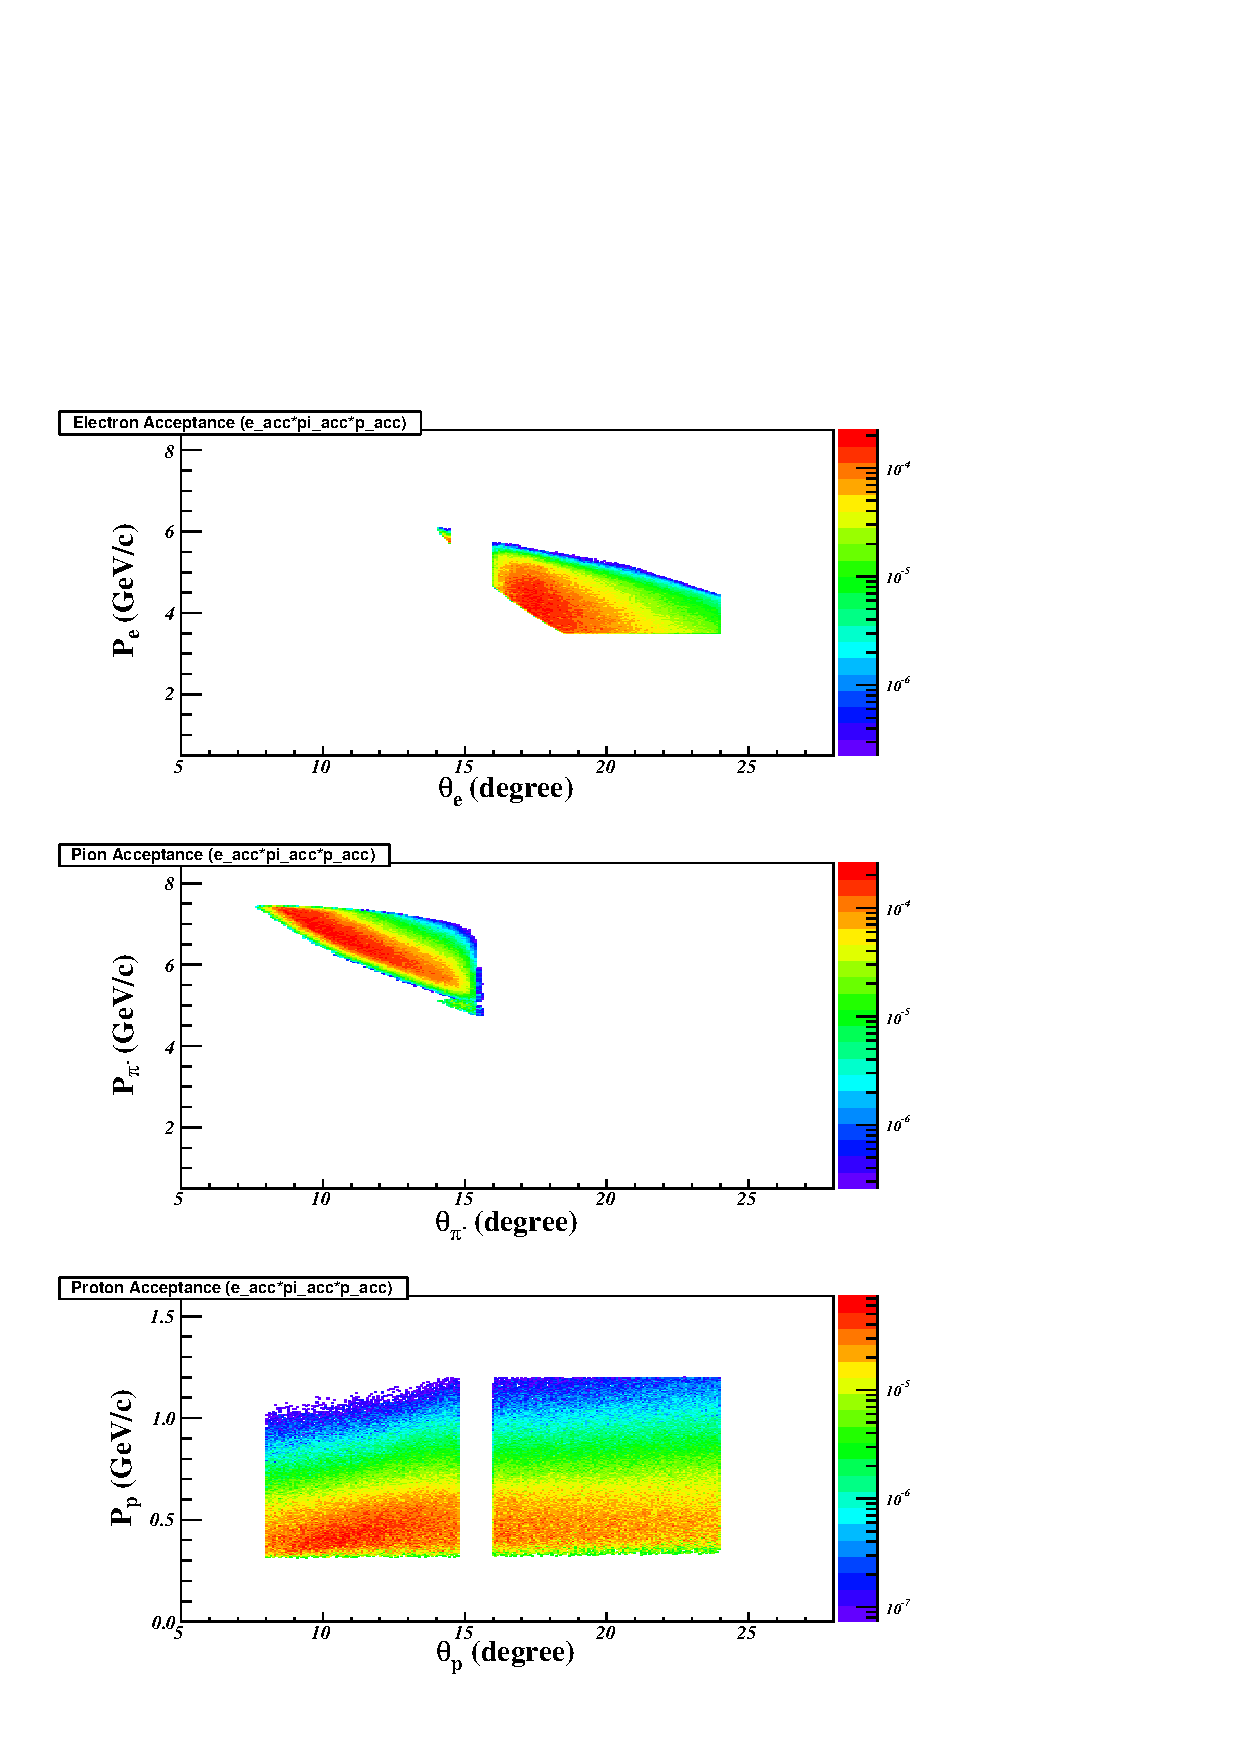
\includegraphics[type=pdf, ext=.pdf,read=.pdf,width=0.35\textwidth]{./figures/E11_acc_epip_Q2gt4}
%    }
%   \caption[The acceptance of the momenta and scattering angles for electrons, $\pi^{-}$ and protons when only detecting small angle protons]{\footnotesize{The acceptance of the momenta and polar angles  at two different $\mathrm{Q^{2}}$ cuts  when only detecting small angle protons with the existing SoLID detectors. In each panel, the top, middle and bottom plots are for electrons, $\pi^{-}$ and protons, respectively. The distribution of protons is given by assuming we detect all recoil protons. Colors correspond to rates (Hz) in log scale.}}
%  \label{p_theta1}
%  \end{center}
%\end{figure}

\begin{figure}[!ht]
 \begin{center}
    \subfloat[w/ PRD]{
      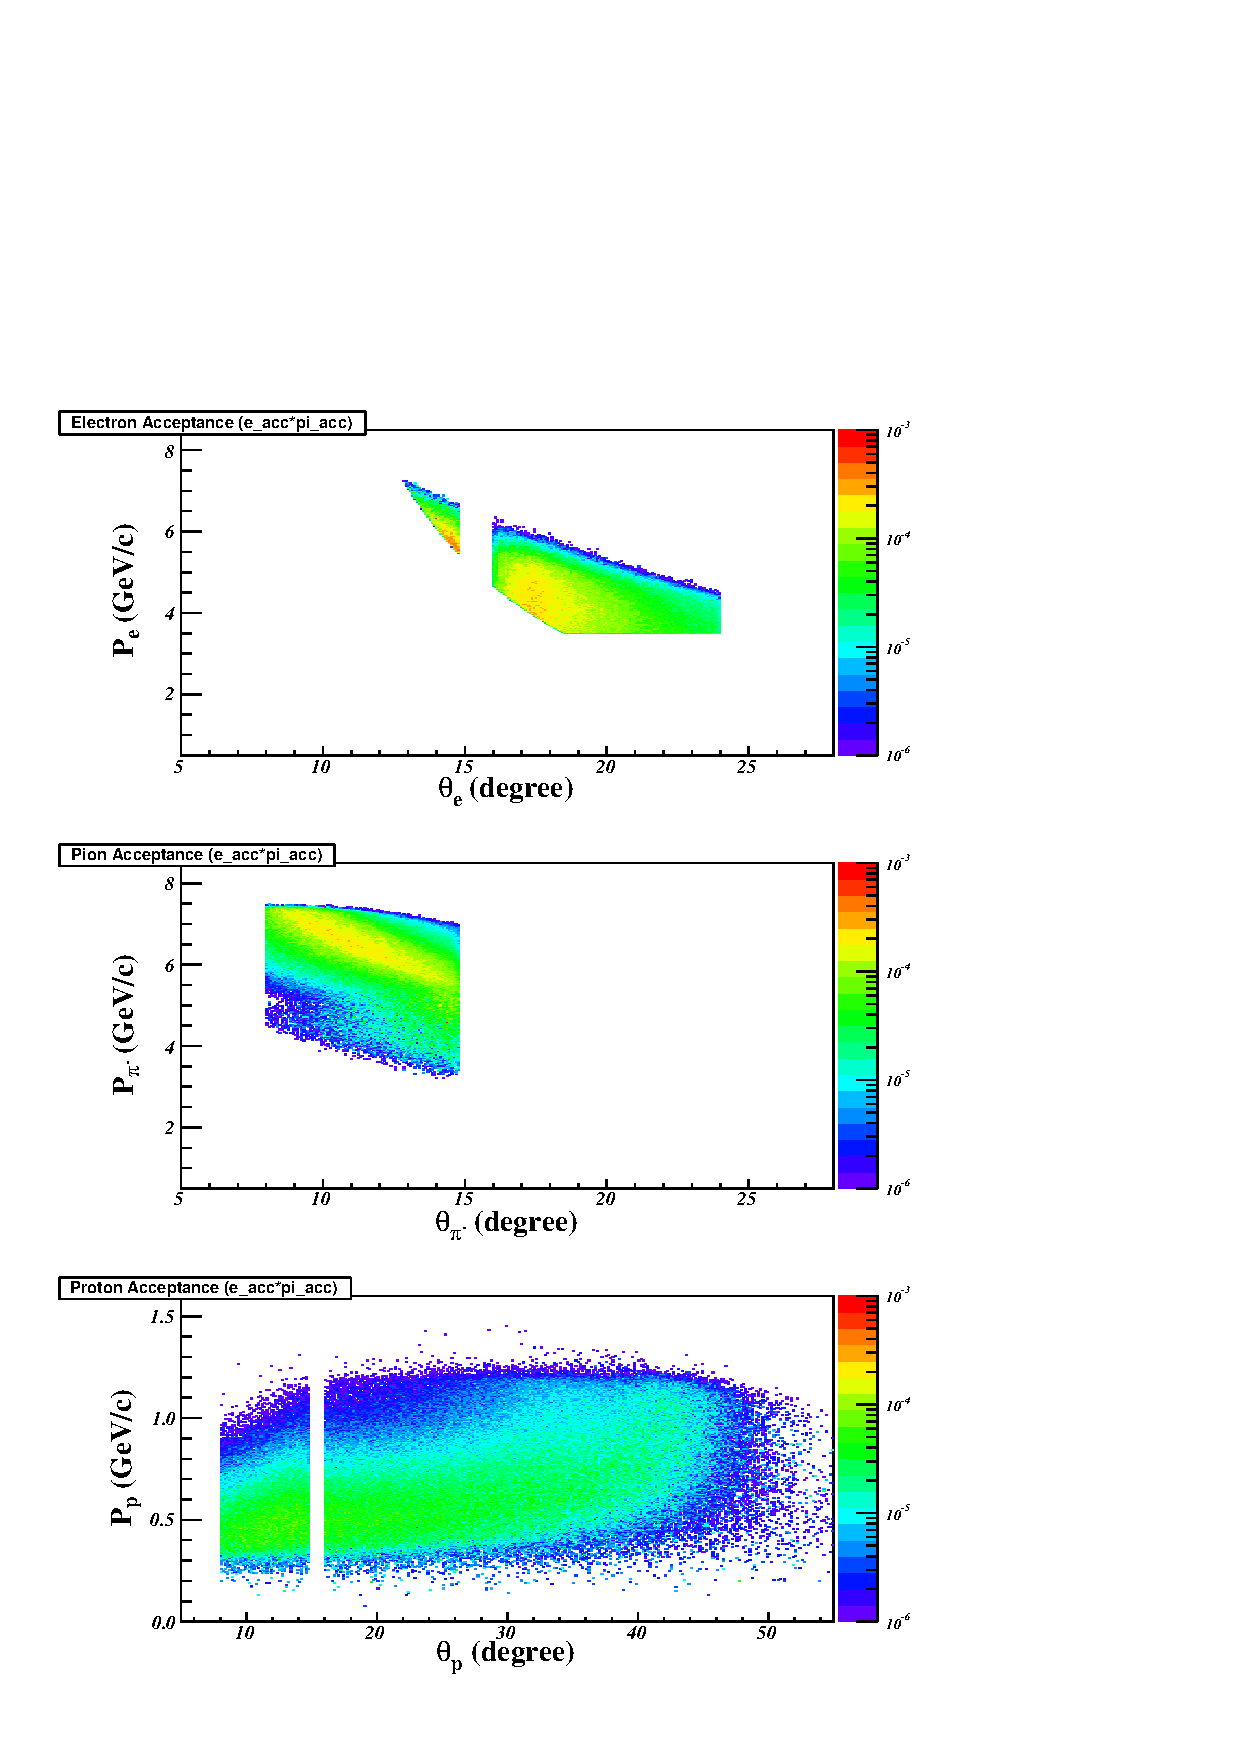
\includegraphics[type=pdf, ext=.pdf,read=.pdf,width=0.35\textwidth]{./figures/E11_acc_epi_Q2gt4}
    }
     \subfloat[w/o PRD]{
      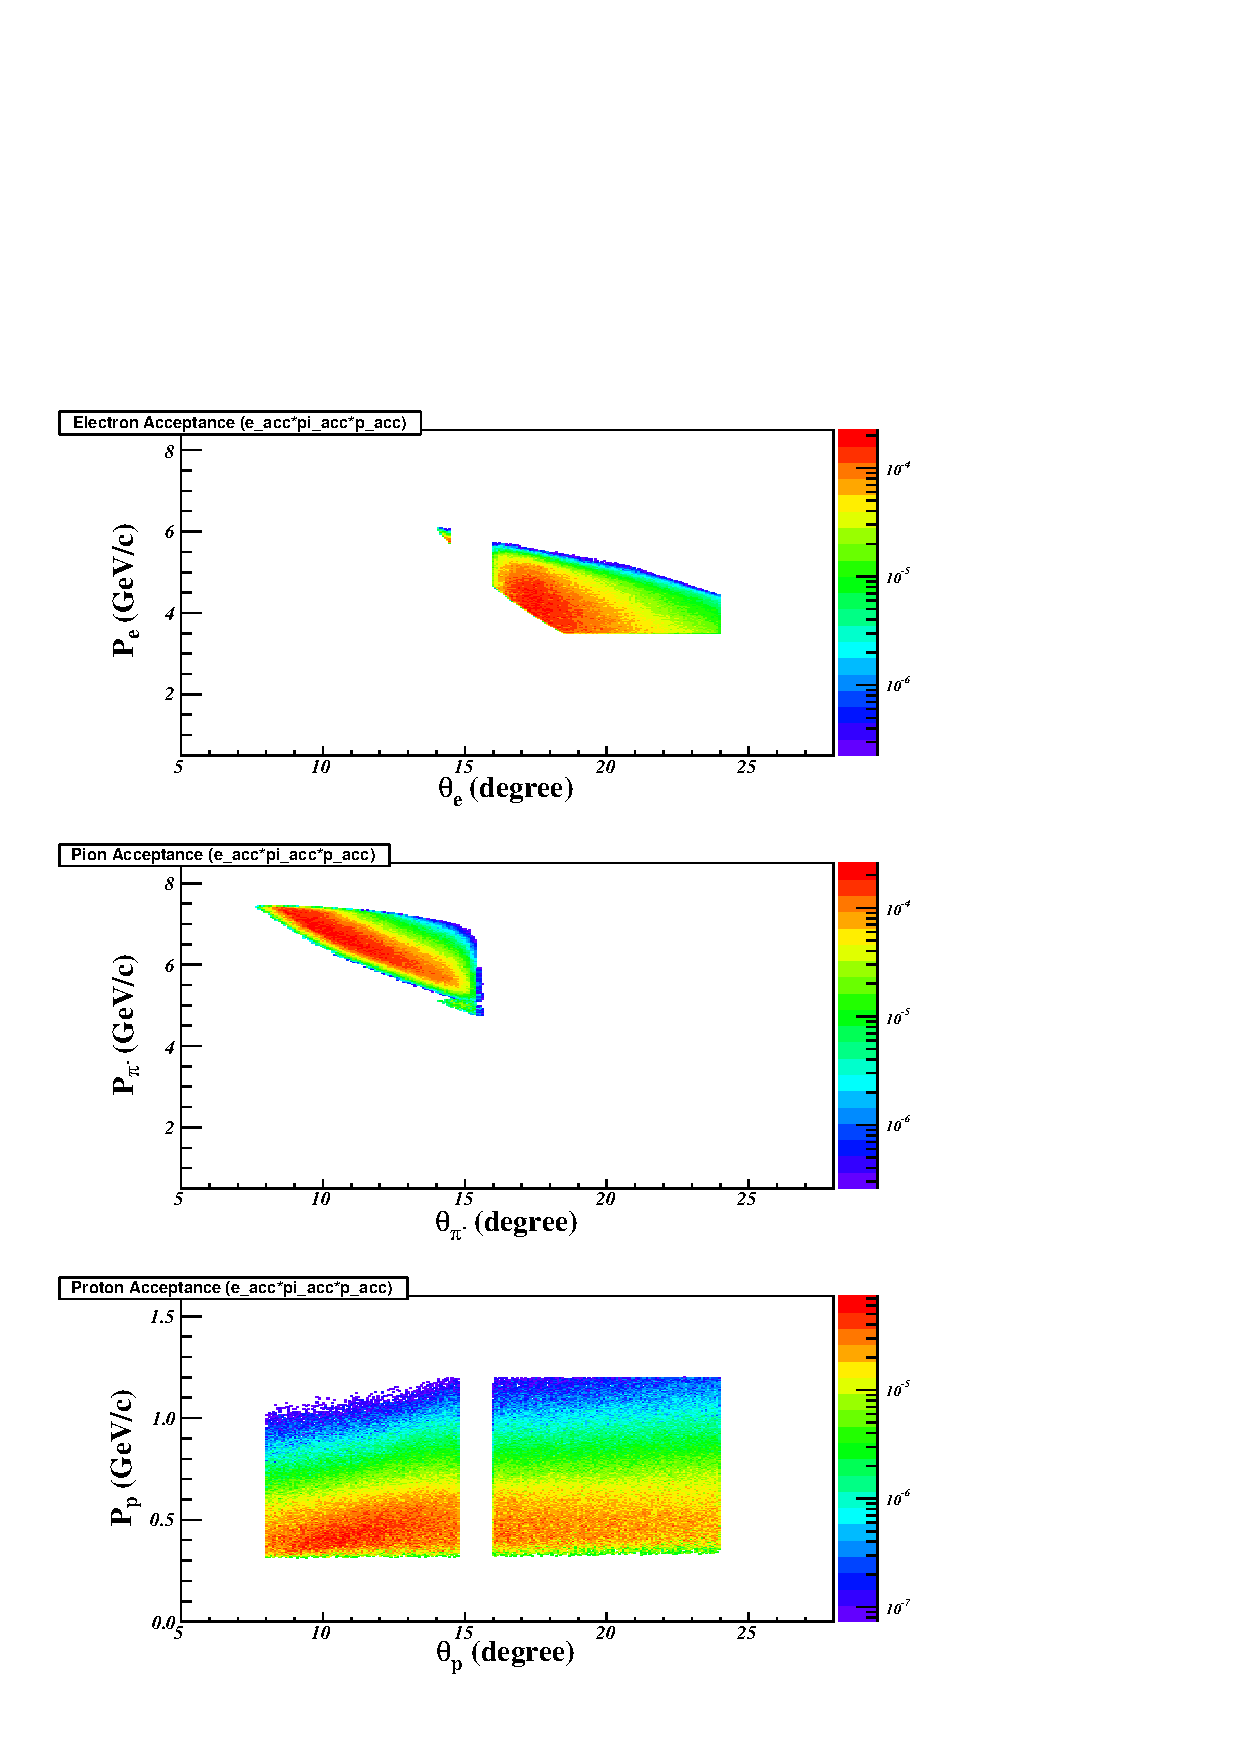
\includegraphics[type=pdf, ext=.pdf,read=.pdf,width=0.35\textwidth]{./figures/E11_acc_epip_Q2gt4}
    }
   \caption[The acceptance of the momenta and scattering angles for electrons, $\pi^{-}$ and protons]{\footnotesize{The acceptance of the momenta and polar angles w/ or w/o the PRD. In each panel, the top, middle and bottom plots are for electrons, $\pi^{-}$ and protons, respectively. A cut of $\mathrm{Q^{2}>4~GeV^{2}}$ is applied. Colors correspond to rates (Hz) in log scale.}}
  \label{p_theta}
  \end{center}
\end{figure}
The kinematic coverage in $Q^{2} vs. x_{B}$ is shown in Fig.~\ref{kin_cor} where two proton detection cases were given: (a) by using  existing SoLID detectors to detect protons at small angles ($8^{\circ}\sim24^{\circ}$) and adding a new proton recoil detector to detect rest of recoil protons at large angle ($24^{\circ}\sim65^{\circ}$), or (b) by only using the existing SoLID detectors. These distributions were weighted by the DVMP cross sections and the spectrometer acceptance obtained from the GEANT4 simulation with the SIDIS configuration. As shown in these plots, the range of $Q^{2}$ is from 1.0~$GeV^{2}$ to 8.0~$GeV^{2}$, $x_{B}$ goes from 0.1 up to 0.75.   

Fig.~\ref{p_theta} shows the momentum and angular acceptance of electrons, $\pi^{-}$ and protons which form the DVMP events and can be detected with the SoLID detectors and (or) with the new PRD . A cut of $\mathrm{Q^{2}>4~GeV^{2}}$ is applied since most of valid DVMP events are at high $Q^{2}$. The recoil protons shown in Fig.~\ref{p_theta}  have low momenta ranged from 0.3~GeV/c up to 1.2~GeV/c and their rates distribute near uniformly along the scattering angle. 

\subsection{Estimated Rates}
\begin{table}[!ht]
\centering
\begin{tabular}{|c|c|c|}
 \hline
  $\mathrm{1<Q^{2}<4~GeV^{2}}$             &    $\mathrm{Q^{2}>4~GeV^{2}}$  & Total\\
 \hline
                  \multicolumn{3}{|c|}{DVMP: $\vec{n}(e,e'\pi^{-})p$ Triple-Coincidence (Hz)}     \\
 \hline
 17.79 (0.22)   &  0.53 (0.31) & 26.45 (7.66)   \\
 \hline
                  \multicolumn{3}{|c|}{SIDIS: $\vec{n}(e,e'\pi^{-})X$ Double-Coincidence (Hz)}                                     \\
 \hline
1388.85 & 35.77 & 1424.62   \\
 \hline
\end{tabular}
\caption[Triple-Coincidence rates for neutron-DVMP]{\footnotesize{Triple-Coincidence  rates for DVMP events compared with the SIDIS rates. Numbers in brackets are the DVMP rates with only detecting protons using existing SoLID detectors. The online production trigger will be the SIDIS double-coincidence trigger of which rates are also given.}}
\label{rate_table}
\end{table} 
Table~\ref{rate_table} lists the triple-coincidence rate of the DVMP events. The rates were calculated with the simulated events weighted by the target luminosity, the SoLID acceptances and cross sections. The rates are the unpolarized event rates and are not corrected by the beam and target polarization, target dilution and so on. The total integrated physics rate is estimated to be around 26~Hz  at 11~GeV, or  0.53 Hz at $\mathrm{Q^{2}>4~GeV^{2}}$. If only using the existing SoLID detectors to detect protons, the rate drops to 0.31 Hz at $\mathrm{Q^{2}>4~GeV^{2}}$.  For comparing,  the table also gives the SIDIS rate  which will be the online production trigger rates and is the main background of the DVMP events. 

\subsection{Asymmetry Projections}
\begin{figure}[!ht]
 \begin{center}
     \subfloat[w/ PRD]{
      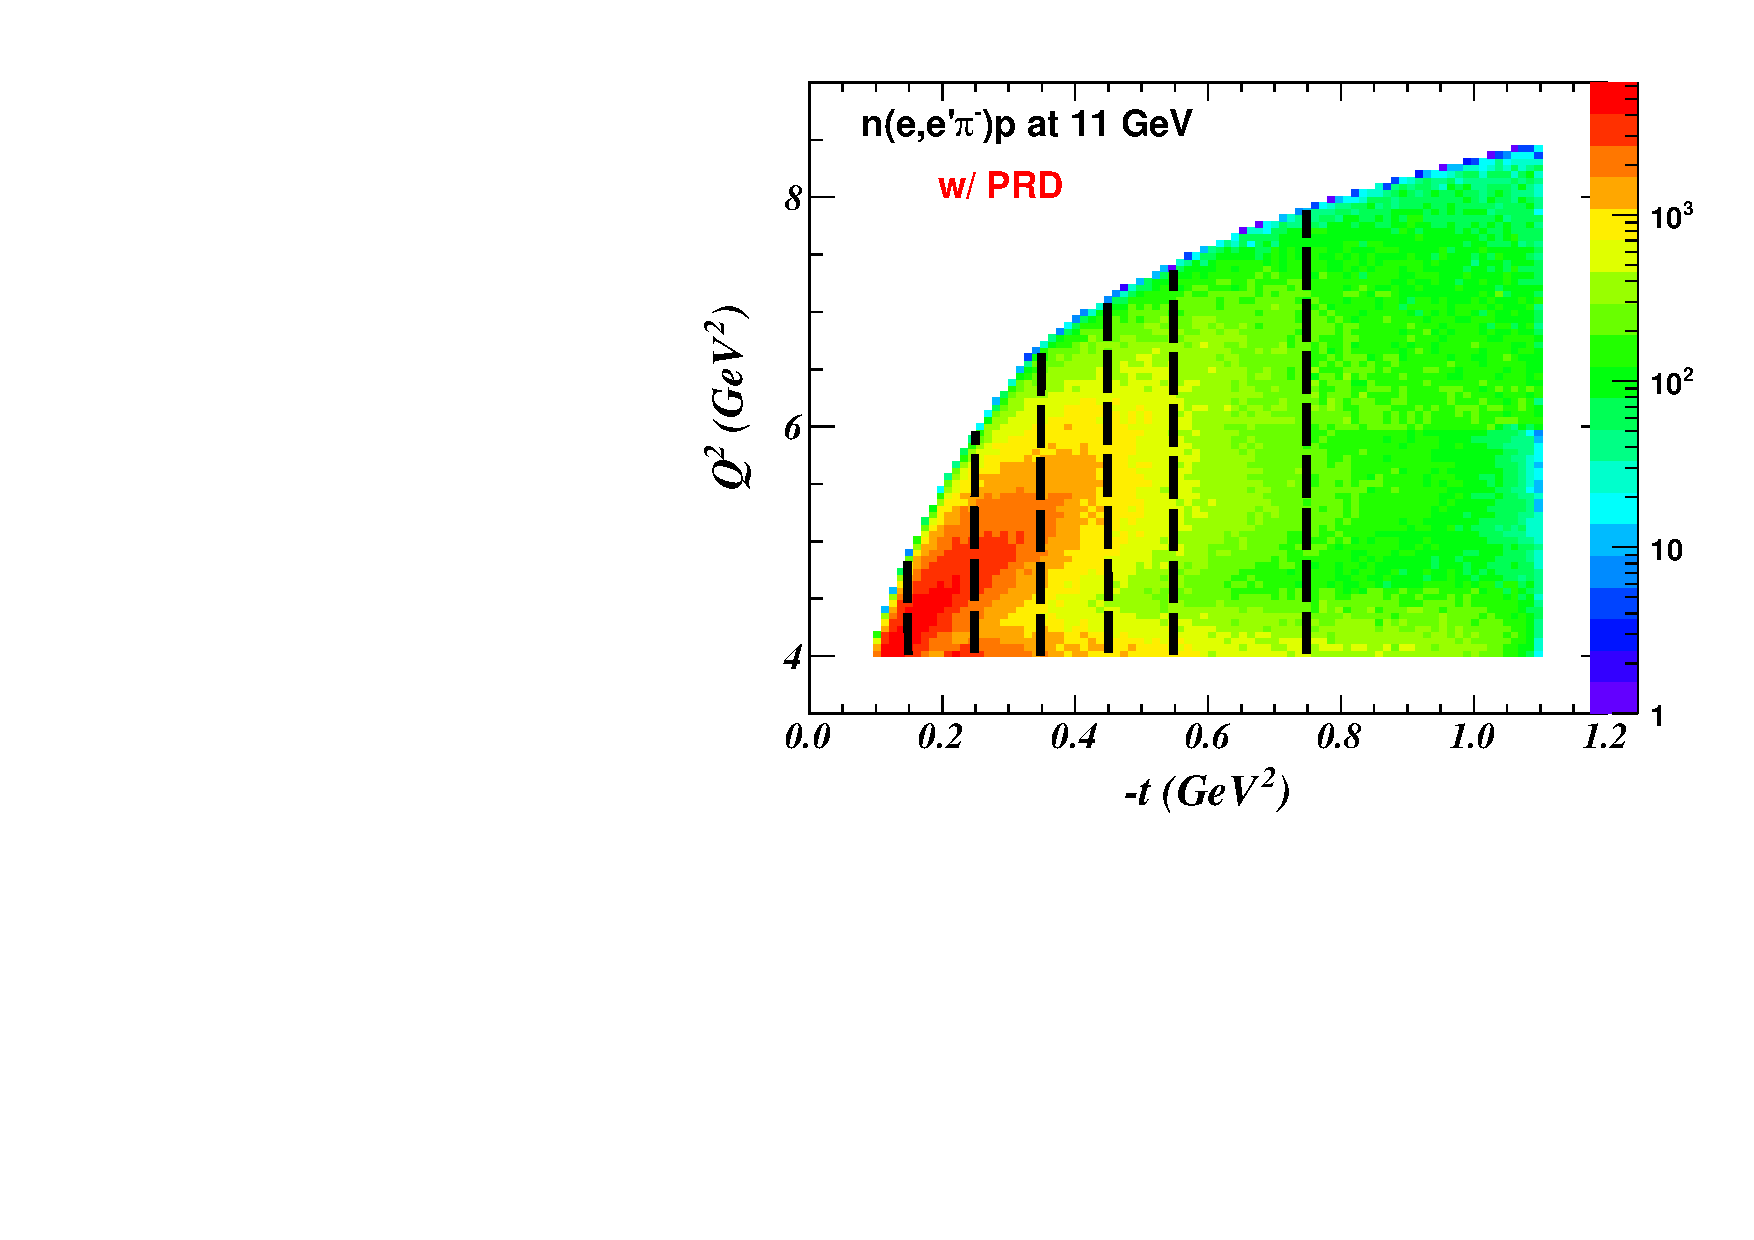
\includegraphics[type=pdf, ext=.pdf,read=.pdf,width=0.5\textwidth]{./figures/E11_Q2_t_bin_prd} }
    \subfloat[w/o PRD]{
      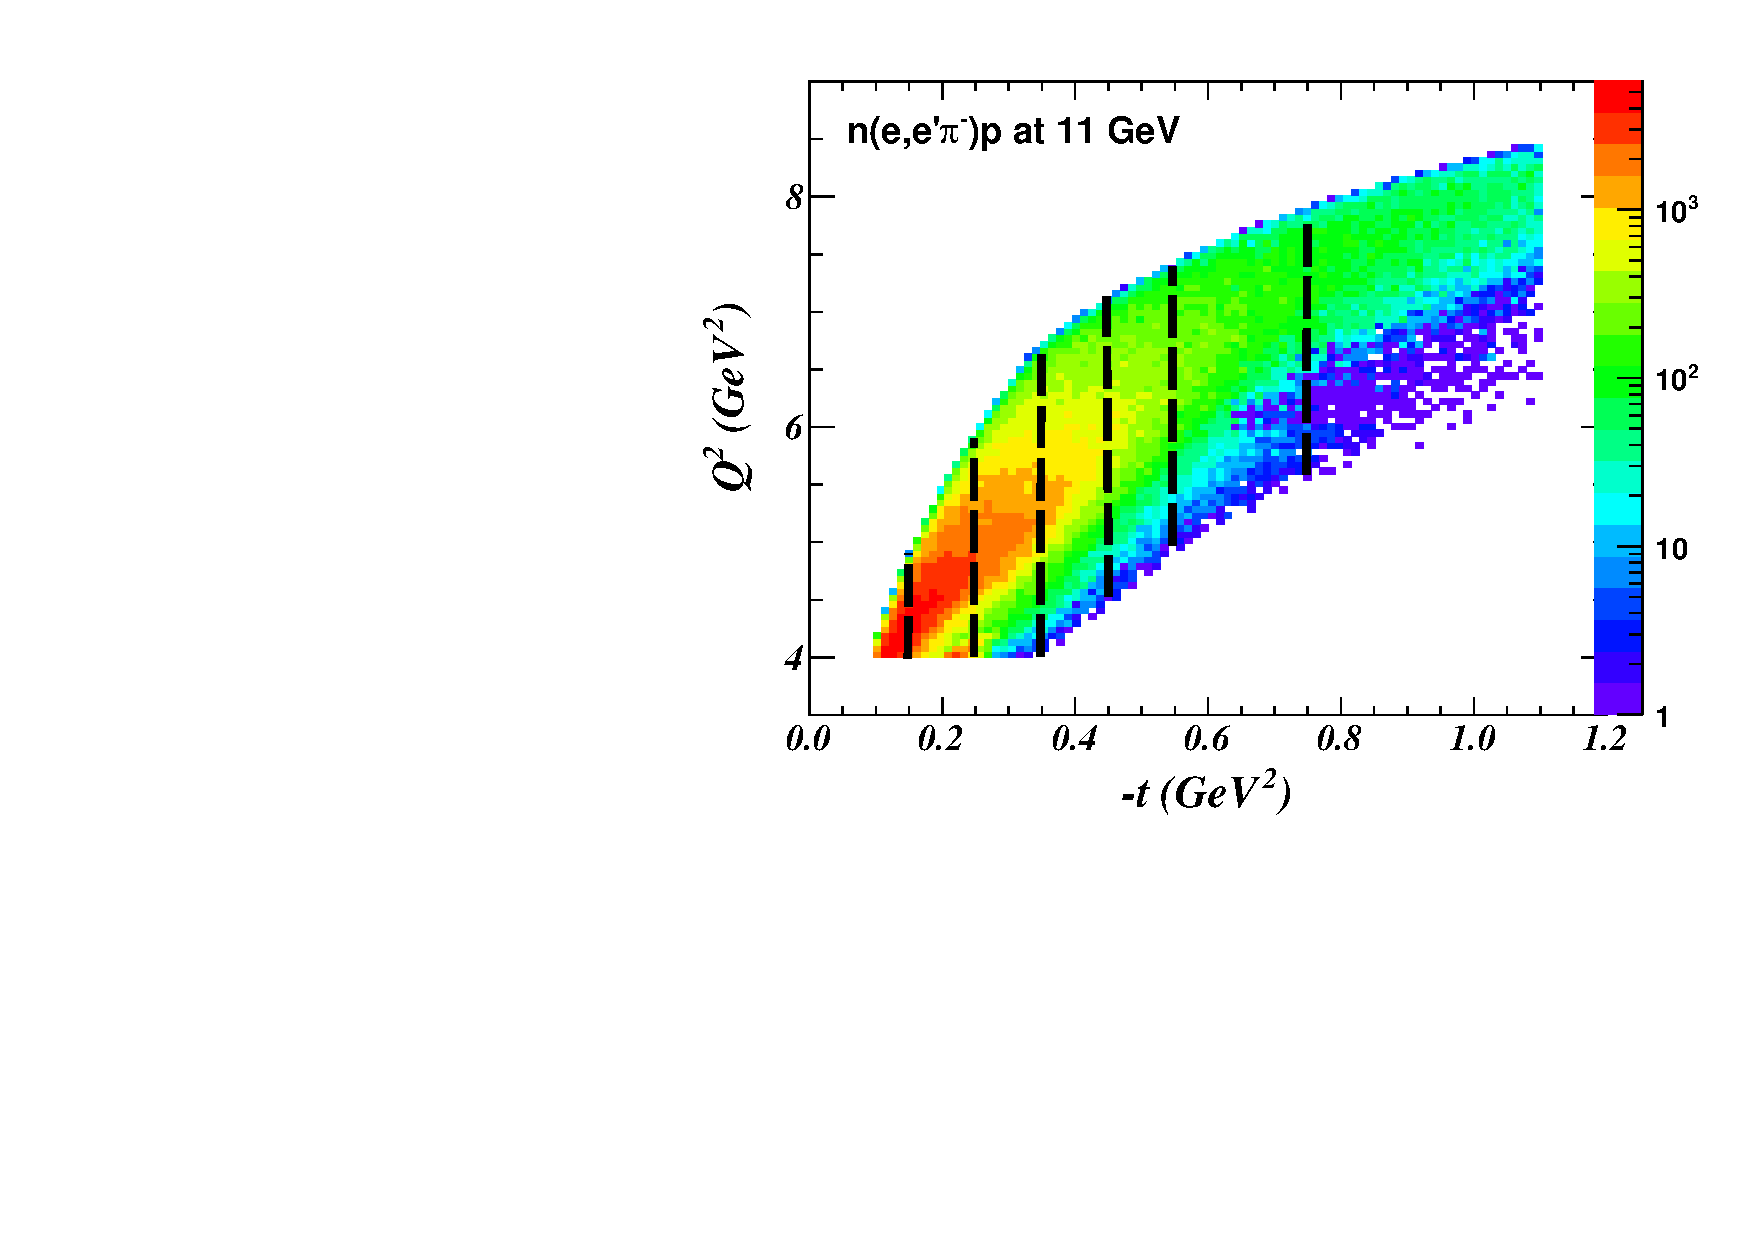
\includegraphics[type=pdf, ext=.pdf,read=.pdf,width=0.5\textwidth]{./figures/E11_Q2_t_bin} }
   \caption[$Q^{2}$ vs. $-t$]{\footnotesize{$Q^{2}$ vs. $-t$ where the black dash lines specify the boundaries of 7 $-t$ bins. The color panel indicates the raw counts with 48 days of beam time at 11 GeV and assuming protons to be detected only by existing SoLID detectors. }}
  \label{Q2_t_bin}
  \end{center}
\end{figure}
The proposed new experiment will run in parallel with E12-10-006 of which total beam time of 48 days at $E_{0}=11~GeV$ has been approved.  As shown in Fig.~\ref{Q2_t_bin}, We defined 7 $-t$ bins of which the the boundaries are defined by the array:
 \begin{equation}
     -t[8] = [0.0, 0.15, 0.25, 0.35, 0.45, 0.55, 0.75, 1.10]~~~~(in~GeV^{2})
 \end{equation}
The number of events ($N_{i}$) in the $i$th bin is calculated with the total simulated events after applying cuts on important kinematic variables, e.g. $Q^{2}>4~GeV^{2}, W>2~GeV, 0.55<\epsilon<0.75 and t_{min}<t<t_{max}$. As shown in Eq.~\ref{ncount}, each event survived the cuts then is weighted by the unpolarized cross section, the acceptance of the electron, pion and photon. $N_{i}$ is further corrected by the phase-space ($PSF$) defined in the event generator to randomly generate a total number of events ($N_{gen}$), beam-time ($T$), the target luminosity ($L=10^{36} cm^{-2}s^{-1}$), and the overall detector efficiency ( $\epsilon_{eff}$):
 \begin{equation}
     N_{i} = (\sum_{j\in i-bin} \sigma^{avg}_{j}\cdot A^{e}_{j} \cdot A^{\pi^{-}}_{j} \cdot A^{p}_{j}) \cdot (PSF/N_{gen}) \cdot T \cdot L \cdot \epsilon_{eff},
     \label{ncount}
 \end{equation}
 where $j$ is the $j$th event in the $i$th bin, $\sigma^{avg}_{j}$ is the cross section of the event. $A^{e(\pi^{-},p)}_{j}$ is the acceptance weight of the electron (pion, proton) in this event. The detector efficiency, $\epsilon_{eff}$, is fixed at 85\%. $N_{i}$ corresponds to the raw experimental count of electrons scattering on neutrons in $\mathrm{^{3}He}$ before taking into account the target polarization ($P\sim60\%$), the effective polarization of neutrons ($\eta_{n}\sim86.5\%$) and the dilution effect from other reaction channels when electrons scattering on $\mathrm{^{3}He}$ ($f \sim 90\%$). The statistical error of the target single spin asymmetry ($A_{UT}$) in each bin can be given as:
  \begin{equation}
    \delta A_{UT} = \frac{1}{P\cdot\eta_{n}\cdot f} \sqrt{\frac{1-(P\cdot <A_{UT}>)^{2}}{N^{+}_{i}+N^{-}_{i}}},
    \label{stat_err}
 \end{equation}
 where $N^{+(-)}_{i}$ is the number of counts in each bin when the target polarization is up (down), and we easily have $N_{i}=N^{+}_{i}+N^{-}_{i}$; $<A_{UT}>$ is the average asymmetry in the bin. As shown in {\bf Section.X},  $A_{UT}$ is predicted with a phenomenological model, but because of not performing a L/T separation in this experiment, the asymmetry should be corrected by another dilution factor which is defined as:
\begin{equation}
  f_{L/T} =\frac{\epsilon\cdot\sigma_{L} }{\sigma_{T}+\epsilon\cdot\sigma_{L} },
\end{equation} 
where $\epsilon=1/(1+\frac{2\nu}{Q^{2}}tan^{2}(\theta))$. Hence, $A_{UT} = f_{L/T}\cdot A_{UT}^{model}$.

\begin{figure}[!ht]
 \begin{center}
      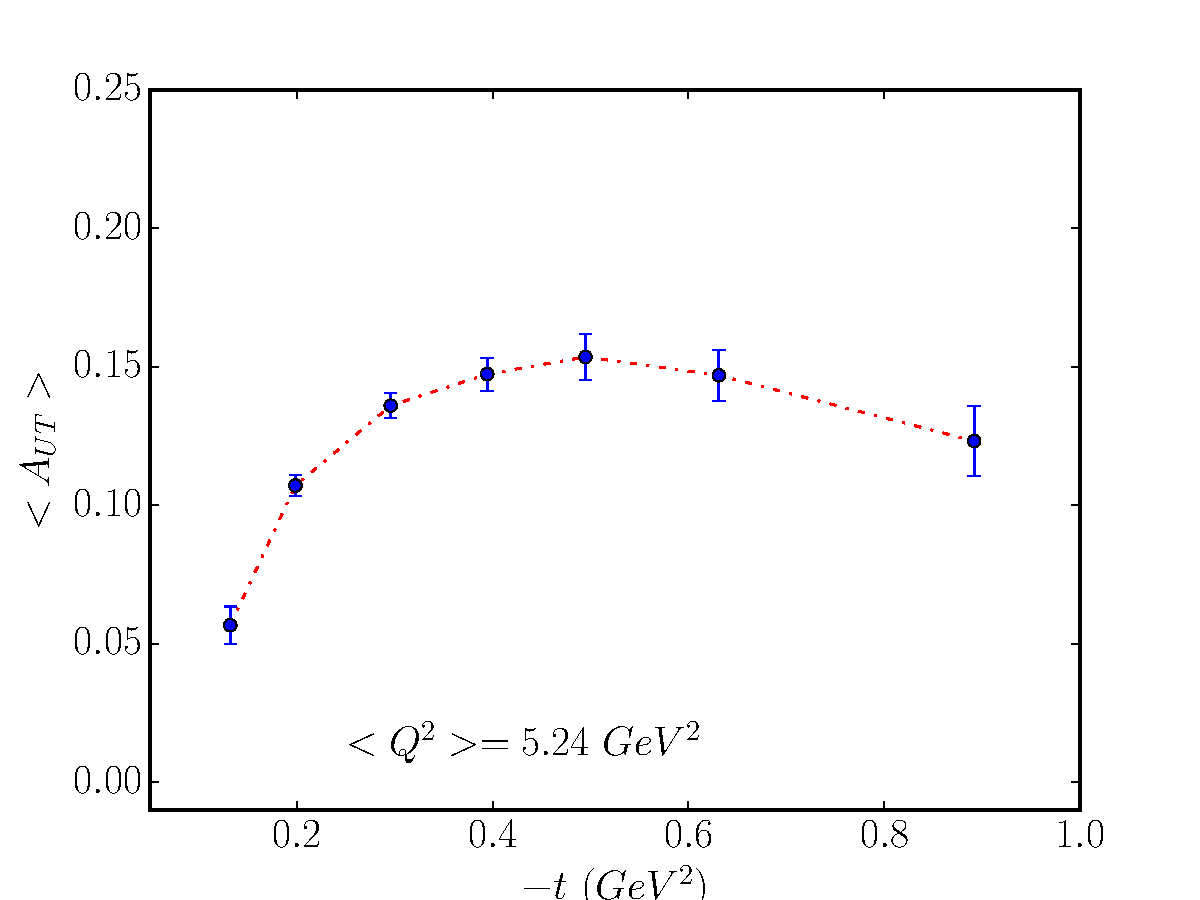
\includegraphics[type=pdf, ext=.pdf,read=.pdf,width=0.7\textwidth]{./figures/bin_asym_t}
      \caption{\footnotesize{Projection of target sing spin asymmetry ($A_{UT}$) in $-t$ binning for DVMP with transversely polarized $\mathrm{^{3}He}$ at $E_{0}=11~GeV$. The error bars are the projected statistical uncertainties defined in Eq.~\ref{stat_err}. The asymmetry value in each bin is predicted with the model given in {\bf Section.X} and is diluted due to not separating the L/T contributions. The left plot shows the projection w/o a new proton recoil detector while the right plot shows a better ojected result with the new detector. One can see the average asymmetries are also changed between two configurations and it is because the asymmetry strongly depends on $Q^{2}$ which changes w/ or w/o the PRD.}}
  \label{asym_t}
  \end{center}
\end{figure}
Fig.~\ref{asym_t} shows the distribution of $A_{UT}$ vs. $-t$ with projected statistical errors discussed above. Compared with the existing HERMES results (Fig.~\ref{fig:hermes_aut}), the new measurement could provide more precious data to be directly compared with theoretical predictions. 

\section{Missing Mass and Background}

\section{Systematic Uncertainties}
\begin{table}[!htp]
\centering
\begin{tabular}{|c|c|}
\hline
{\bf Sources}                  & {\bf Relative Value} \\\hline
Beam Polarization              & $2\%$ \\\hline 
Target Polarization            & $3\%$ \\\hline 
Acceptance                     & $3\%$ \\\hline
$\pi^{0}$ Contamination        & $<5\%$  \\\hline
Other Contamination            & $<5\%$ \\\hline
Radiation Correction           & $1\%$ \\\hline
\end{tabular}
\caption{\footnotesize{Expected systematic errors.}}\label{table:det_sys_err}
\end{table}
The detector related systematic errors are expected to be similar to the ones given in the E12-10-006 proposal as well as in other SIDIS experiments with SoLID, as shown in Table~\ref{table:det_sys_err}. The systematic error of the $\pi^{0}$ correction procedure and other background subtraction will be controlled at the 1\%$\sim$5\% level. %Meanwhile, it is still an ongoing effort to understand and estimate the systematic errors from fitting the CFFs with the asymmetries. 
We expect to provide a full list of systematic errors in the proposal. 
